\chapter{Realization}

\begin{multicols}{2}
  Because the \acrshort{qaas} web application itself is already built on top of existing frameworks, libraries, and technologies, the
  integration of the SentinelOne was relatively straightforward. The \acrshort{api} itself is well-documented, and the \acrshort{npm}
  package provided by SentinelOne is easy to use. The only challenge was to understand the data structure of the SentinelOne, choosing
  the right and more important data to display, modelling it in the \acrshort{qaas} database, and then
  displaying it in the web application.

  \section{The Back-end}

  As stated before, \acrshort{qict} wishes to utilize the 2nd generation of Firebase Cloud Functions, therefore a new Firebase project
  was created and stored on the cloud (\textit{using Azure DevOps}). The author also needs to make a decision in regards on how the
  infrastructure of the codebase should be structured. Because \acrshort{qict} is always critical and open to feedback, the author is
  given access to the old Firebase codebase (\textit{utilizing version 1.0}), and find any potential upsides and downsides of that
  project repository. The author then, by an informed decision, is allowed to decide whether to structure the new codebase in the same
  way as the old one. The author has certainly decided to create some new adjustments to the new codebase. For example, instead of
  stacking all functionalities that a Firebase Cloud Function might have, the author has decided to improve the codebase especially
  regarding the separation of concerns. Specifically, the response from the \acrshort{api} is modelled using Interfaces and Classes
  object within the Models directory, allowing for a consistent reuse across different functions. Additionally, distinct Routers
  and Controllers directories has been established, each with specific responsibilities. The Routers directory primarily handles
  external communications with the \acrshort{api}, utilizing \texttt{Axios} (\textit{\cite{axiosNpm}}) for handling the GET requests.
  The Controllers directory, contains the back-end logic of the cloud function, bridging Models and Routers and ensuring comprehensive
  error documentation. This structure defines the behavior of the Firebase Cloud Function version 2.0 of the \acrshort{qaas} app.

  Moreover, there are Utilities and Middlewares directories, which are used to handle common functionalities and errors. The Utilities
  directory contains functions that are used across the codebase, such as logging errors, and the Middlewares directory contains functions
  that are used to handle the request and response of the cloud function. For example, the \texttt{logError} function in the Utilities
  directory is used to log errors in the console, and the \texttt{handleError} function in the Middlewares directory is used to handle
  errors in the response of the cloud function. This structure allows for a more organized and maintainable codebase.

  The types of functions that are used throughout the project are the following:
  \begin{itemize}
    \item \texttt{onCall}: This type of function is used to handle callable functions, which are called from the client-side. It is used
          to handle requests from the client-side. This is the main function in which the SentinelOne data is fetched and processed.
    \item \texttt{onRequest}: This type of function is used to handle \acrshort{http} requests, which are called from the client-side.
          It is mainly for initial testing, as setting this function up is easier and faster. However, the author does not recommend
          using this in the production, as it lacks authentication and security for the end-user.
    \item \texttt{onSchedule}: This type of function is used to handle scheduled functions, normally called cron-jobs, which are called
          at a specific time. It is used to handle scheduled tasks that need to be executed at a specific time. There is only one
          scheduled function in the project, which is used to replace the old SentinelOne \acrshort{api} key with a new one that is
          securely stored in Google Secret Manager, therefore ensuring proper connection and access to the secret vault, every month.
  \end{itemize}

  \subsection{Setting up permissions with Google Secret Manager}

  Because every call to the SentinelOne \acrshort{api} requires an authorization through a valid SentinelOne \acrshort{api} key, it is
  crucial to store this key securely on the Internet, where not everyone can access it. Following the guideline from the Company
  Supervisor, in whom is not a big fan of storing sensitive information in .env files or directly in the code, the author stored the
  SentinelOne \acrshort{api} key in a Secret within Google Secret Manager. The number one reason as to why is because Firebase Cloud
  Functions work well with Secret Manager, as they are both Google Cloud products. Therefore, the author can easily edit the settings of
  a specific cloud function to have access to the latest version of a specific Secret, providing that they are stored within the same
  project directory.

  \subsubsection{Service Account}

  The first crucial step in setting up the permissions with Google Secret Manager is to create a Service Account. A Service Account is
  a special type of Google account that belongs to the application or a virtual machine, instead of to an individual end-user. It is
  used to operate and manage services without sharing user credentials (\textit{\cite{serviceAccounts}}). Whenever a function is created
  in Firebase, it is automatically assigned a Service Account, the admin can edit the permissions of the Service Account to have access
  to the Secrets stored in the Secret Manager. With the proper access level granted to a specific Service Account assigned to a desired
  function, the author can then easily configure on which Secrets his cloud functions can have access to.

  \subsection{Compliance with ESLint compiler}
  Lastly, the back-end project utilizes Node.js as the runtime environment, with \acrshort{ts} as the programming language. This has
  caused longer compilation time as it involves additional steps like type checking and transpiling the code to \acrshort{js}. However,
  it is still believed to be the better practice as  \acrshort{js} in  nature is a loosely typed language, and it is easy to make mistakes
  in the code as its variables do not have a fixed type. While this sometimes can be beneficial as it makes the development faster and
  more flexible, it also introduces challenges, particularly in debugging and maintaining the code. To prevent this, both the author and
  the Company Supervisor have decided to use and adhere to \acrshort{ts} and ESLint rules, to ensure static typing, code quality and
  consistency to the coding standards.
\end{multicols}

\begin{lstlisting}[language=JavaScript, caption={Example of Class and Interface defined in Models}]

  export interface Customer {
    customerId: string;
    customerName: string;
    orgUnitType: string;
    parentId: string;
    city: string;
    stateProv: string;
    country: string;
    county: string | null;
    postalCode: string;
    contactEmail: string;
  }
  
  /**
   * Class for CustomerModel.
   */
  export class CustomerModel {
    private readonly firestore: FirebaseFirestore.Firestore;
    private readonly collectionName = "customers";
    private readonly context = "CustomerModel";

    constructor() {
      this.firestore = admin.firestore();
    }

    serializeCustomerToJson(customer: Customer): string {
      return JSON.stringify(customer);
    }
  
    /**
     * Deserializes a JSON string to a Customer object.
     * @param {string} json The JSON string to deserialize.
     * @return {Customer} The deserialized Customer object.
     */
    deserializeJsonToCustomer(json: string): Customer {
      return JSON.parse(json) as Customer;
    }
  
    /**
     * Creates a new customer in Firestore.
     * @param {Customer} customer Customer to add to Firestore.
     * @return {Promise<FirebaseFirestore.DocumentReference<FirebaseFirestore.DocumentData>> | undefined}.
     */
    async createCustomer(customer: Customer): Promise<FirebaseFirestore.DocumentReference<FirebaseFirestore.DocumentData> | undefined> {
      try {
        return this.firestore.collection(this.collectionName).add(customer);
      } catch (ex: unknown) {
        logError(ex, this.context + ".createCustomer");
      }
      return undefined;
    }
  
    /**
     * Retrieves a customer by its ID from Firestore.
     * @param {string} customerId The ID of the customer to retrieve.
     * @return {Promise<Customer | undefined>} A promise that resolves with the customer object if found, or undefined if not found or 
     an error occurs.
     */
    async getCustomer(customerId: string): Promise<Customer | undefined> {
      try {
        const doc = await this.firestore.collection(this.collectionName).doc(customerId).get();
        if (!doc.exists) {
          return undefined;
        }
        return doc.data() as Customer;
      } catch (ex: unknown) {
        logError(ex, this.context + ".getCustomer");
        return undefined;
      }
    }
  
    /**
     * Updates an existing customer in Firestore.
     * @param {string} customerId The ID of the customer to update.
     * @param {Partial<Customer>} customer The partial customer object containing updates.
     * @return {Promise<void>} A promise that resolves when the update is complete.
     */
    async updateCustomer(customerId: string, customer: Partial<Customer>): Promise<void> {
      try {
        await this.firestore.collection(this.collectionName).doc(customerId).update(customer);
      } catch (ex: unknown) {
        logError(ex, this.context + ".updateCustomer");
      }
    }
  
    /**
     * Deletes a customer from Firestore.
     * @param {string} customerId The ID of the customer to delete.
     * @return {Promise<void>} A promise that resolves when the customer is successfully deleted.
     */
    async deleteCustomer(customerId: string): Promise<void> {
      try {
        await this.firestore.collection(this.collectionName).doc(customerId).delete();
      } catch (ex: unknown) {
        logError(ex, this.context + ".deleteCustomer");
      }
    }
  }  
\end{lstlisting}

\begin{lstlisting}[language=JavaScript, caption={An example of Firebase HTTP Request onCall Cloud Function version 1.0}]
  import * as functions from "firebase-functions";
  import * as admin from "firebase-admin";
  import { Secrets } from "../Firebase/Secrets";
  import { FirebaseCall } from "../Firebase/FirebaseCall";
  import axios from 'axios'; 

  export default functions
    .region("europe-west1")
    .https.onCall(async (data, context) => {
        try {
          // context.app will be undefined if the request doesn't include a valid
          // App Check token.
          if (context.app === undefined) {
            throw new functions.https.HttpsError(
              "failed-precondition",
              "The function must be called from an App Check verified app."
            );
          } 
        } catch (error) {
          console.error("An error occurred in the Firebase HTTP Request onCall Cloud Function: ", error);
          throw new functions.https.HttpsError("internal", "An error occurred while processing the request.");
        }
  });
\end{lstlisting}

\begin{lstlisting}[language=JavaScript, caption={onCall Cloud Function version 2.0, where the parameters of the function is less and 
  the way it handles the authorization is different}]
  import axios from "axios";
  import * as functions from "firebase-functions/v2";
  import { CallableRequest } from "firebase-functions/v2/https";
  import admin from "firebase-admin";

  import { region, sentinelOneURL, sentinelOneApiVersion } from "../../../config";
  import { logError } from "../../../Middleware/LogError";
  import { getSecret } from "../../../Util/Secret";

  export const getSentinelOneData = functions.https.onCall({ region: region }, async (context: CallableRequest<any>) => {
    try {
      // Authentication check
      if (!context.auth) {
        throw new functions.https.HttpsError("unauthenticated", "The function must be called while authenticated.");
      }
      const data = context.data;
  
      // // Checking if the request contains the necessary data
      if (!data || !data.siteId || !data.userId || !data.dataType) {
        throw new functions.https.HttpsError("invalid-argument", "The necessary requirement(s) are missing or invalid in your request.");
      }  
    } catch(ex: unknown) {

    }
  });
\end{lstlisting}

\begin{lstlisting}[language=JavaScript, caption=LogError functionality in the Utilities folder]
  export function logError(error: unknown, context: string): void {
    if (isAxiosError(error)) {
      // AxiosError object, log detailed request and response information
      console.error(`[${context}] Axios error occurred: ${error.message}`);
      console.error(`Response data: ${error.response?.data}`);
      console.error(`Status code: ${error.response?.status}`);
      console.error(`Headers: ${JSON.stringify(error.response?.headers, null, 2)}`);
    } else if (error instanceof Error) {
      // Standard Error object, log message and stack
      console.error(`[${context}] An error occurred: ${error.message} \n Stack: ${error.stack}`);
    } else {
      // Non-Error object, log with a generic message
      console.error(`[${context}] An unknown error occurred:`, error);
    }
  }
\end{lstlisting}


\begin{lstlisting}[language=JavaScript, caption={An example of how that utility is used in the Cloud Function, the reason why exception 
  type is unknown is to comply with the ESLint rules that does not recommend to use the any type to the variables}]
  try {

  }
  catch (ex: unknown) {
    console.log(`An error occured in the getFirestoreData function: ${ex}`);
    logError(ex, "getFirestoreData");
  } finally {
    throw new functions.https.HttpsError("internal", "An error occurred while getting the data in Firestore.");
  }
\end{lstlisting}

\begin{lstlisting}[language=JavaScript, caption={Example of challenges in JavaScript because of its loosely typed nature that creates 
  lack of type safety, type coercion, and type conversion}]
  function add(a, b) {
    return a + b;
  }
  console.log(add(5, '2')); // "52" instead of 7
\end{lstlisting}

\begin{lstlisting}[language=DOS, caption={Another example of JavaScript challenges}]
    C:\Users\ChristopherSulistiyo>node
    Welcome to Node.js v22.1.0.
    Type ".help" for more information.
    > true === 1
    false
    > true + true + true === 3
    true
    > 0 == "0"
    true
    > "0" ==- null
    true
    > -null
    -0
    > -0 == "0"
    true
    > parseInt(0.00000005)
    5
    > typeof(NaN);
    'number'

    > let a = []
    undefined
    > a.length == a
    true
  \end{lstlisting}

\begin{multicols}{2}

  \subsection{SentinelOne NPM packages}
  \acrshort{npm} packages are a necessary component when developing a project in JavaScript, as they are used for managing dependencies
  in Node.js projects. Below are the \acrshort{npm} packages that are used in the project:

  \begin{itemize}
    \item
  \end{itemize}


  \subsection{Firestore database structure}

  Inside the Firestore, there are various collections (tables) that hold different data. Most of the collections are used to store the
  data that is fetched from the SentinelOne \acrshort{api}, and one collection is used to store the user's session and preference data.
  SentinelOne data itself is divided into 2 categories: general SentinelOne data and specific data, both of them can have varying fields
  depending on how SentinelOne structures the data in its \acrshort{json} format. General SentinelOne data only have 1 specific field
  in common, which is the siteId. The idea is to store all the clients' data in one collection, therefore to differentiate the data
  based on client's company, an index of client's site ID (which is unique from each other) is used to separate the data.

  The second category is the specific SentinelOne data, win which the data is not only belong to a specific site ID, but also to a
  specific ID from another SentinelOne data. For example, each threat cam have their own unique timeline of events that have happened.
  Therefore, another field is required that is used as a second index to reference the desired data. The first and second category will
  then have different logic in the cloud function to fetch the data.

  \subsubsection{User Preference}

  A special table in Firestore is created to store the user's preference, each document' ID is the user's ID, therefore ensuring
  uniqueness. In a document, there are 3 different fields:

  \begin{itemize}
    \item timestamp: containing date time in the format of timestamp. It is used as a reference for the Cloud Function to know when is
          the data last updated, and if it exceeds a certain threshold, the Cloud Function will fetch the data from the SentinelOne
          \acrshort{api} again. This will be the field that the fetching cloud function needs to do its if-check first to determine if
          the data is outdated.
    \item widgetIds: containing an array of strings, each string is the ID of the widget that the user wants to see in the dashboard.
          This is used for the convenience of adding, updating, and deleting widgets.
    \item widgetTitle: containing also an array of strings, which serves as the title that the user choose for their widgets. A widget
          title can have the same name as another widget, as long as the widget ID is different.
    \item widgets: containing a map of 3 different fields:
          \begin{itemize}
            \item category: containing a string, which is the category of the widget. The category is used to group the widgets in the
                  dashboard, so the user can easily find the widgets that they want to see. Currently, there are 3 categories: "Threats",
                  "Endpoints", "Applications", and "Miscellaneous". In the future, additional 2 categories can be added: "Ranger
                  (Network Discovery)" and "Rogues". Ranger is a feature that is used to discover the network of the client's machine,
                  and Rogues is a feature that is used to detect any unauthorized devices that are connected to the client's machine.
                  These 2 features are currently deactivated in the \acrshort{qict} site environment for internal reasons, thus the
                  author does not include them in the project.
            \item graphicType: containing a string, which is the type of the graphic that the user wants to see in the widget. Currently,
                  the graphics that the user can utilize are: "Doughnout", "Pie Chart", "Vertical Bar", "Stacked Vertical Bar",
                  "Horizontal Bar", "Stacked Horizontal Bar", "Line Chart", "Scatter", "Bubble", "Pyramid", "Funnel", and "Table".
            \item widgetType: Inside the 4 main categories, the selection is further divided into separate types according to which
                  categories that wanted to be visualized. Agent category can show the status of the agents, such as the number of agents
                  that are connected, disconnected, or in quarantine. Threats category can show the status of the threats that are
                  detected by SentinelOne, such as the number of threats that are detected, resolved, or in quarantine. Applications
                  category show the number of outdated applications that can potentially be a threat to the client's machine, according
                  to the latest \acrshort{cve}s from the \acrshort{nist} and MITRE. The widget categorization is divided as follows:
                  \begin{itemize}
                    \item Endpoint: Agent versions, pending updates, agent by \acrshort{os}, console migration status, domains,
                          encrypted applications, endpoint connected to management, connection status, endpoint health, endpoint list,
                          endpoint summary, installers, load saved filters, local configurations, location IDs, machine types, manual
                          actions required, network health, \acrshort{os} arch, pending uninstall, and scan status.
                    \item Threats: Analyst verdicts, confidence levels, engines, external ticket exists, failed actions, incident status,
                          initiator, mitigated preemptively, note exists, pending actions, reboot required, threat classification,
                          threat list, threat status, threat summary of the week, and unresolved.
                    \item Applications: Risk levels, and most impactful applications according to SentinelOne Vulnerability Score.
                    \item Miscellaneous: SentinelOne news feed, and free text.
                  \end{itemize}
          \end{itemize}

          \subsection{Setting up permissions with Firestore}

          This has got to do with the Firestore database and the access level of permission that a Firebase Cloud Function has. In the
          SentinelOne integration project, the table that contains SentinelOne data cannot be changed by the client, only by fetching new
          data from the SentinelOne \acrshort{api} and replacing the old data. Therefore, only one table remains that actually can be
          changed accordingly by the user, the User Preference table. This table can be changed freely by the user as long as they remain
          logged in to the \acrshort{qaas} app.
  \end{itemize}
\end{multicols}

\begin{figure}[htbp]
  \centering
  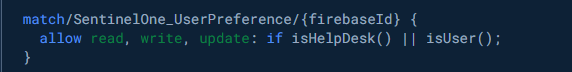
\includegraphics[width=0.8\textwidth]{Figures/User Preference.png}
  \caption{Granting access of read, write, and update from User Preference collection to users in the Firebase Console}
\end{figure}

\begin{multicols}{2}
  \subsection{Connection to Algolia}

  As originally stated, the author and Company Supervisor directly intended on using Algolia search as the SentinelOne \acrshort{api}
  search, although far from being bad, does have type intolerance.

  \section{The Front-end}

  In the front-end side of this project, it is just a matter of calling the Cloud Functions, modelling the \acrshort{json} response
  coming from the Cloud Functions (whether it is from Firestore or SentinelOne), making the visualization graphs using the available
  Flutter package, setting the logic on how to navigate between pages passing the correct data, the logic for how to display the data
  correctly in paginated data tables and visualization widgets, and lastly, the searching, filtering, and filtering functionality.

\end{multicols}
